% !TeX spellcheck = fa-IR
\chapter{نسخه‌های مختلف مسئله}
\label{chapter:varients}
در میان پژوهش‌های مختلفی که روی 
\picod
انجام شده است یکی از مسیرهای پژوهشی تعریف نسخه‌های جدیدی از مسئله است. همانطور که با منعطف کردن گیرنده‌ها، از مسئله‌ی
\icod
به
\picod
رسیدیم می‌توانیم با تغییر در صورت‌بندی
\picod
به مسائل جدید برسیم.

در این فصل با ۴ نسخه دیگر آشنا می‌شویم که هر کدام با تغییر در شرایط مسئله، مسئله‌ای جدید تعریف می‌کنند که کاربردی متفاوت دارد. در بخش اول با افزایش میزان منعطف بودن گیرنده‌ها، مسئله‌ی
\transf{کدگذاری اندیس بسیار منعطف}{very pliable index coding}
 تعریف می‌شود. در بخش دوم با در نظر گرفتن اولویت بین پیام‌ها برای گیرنده‌های مختلف، مسئله‌ی
 \transf{کدگذاری اندیس منعطف ترجیحی}{Preferential Pliable Index Coding}
 را تعریف می‌کنیم. در بخش سوم با حذف فرستنده‌ی مرکزی، گیرنده‌ها به صورت محلی اطلاعات خود را به اشتراک می‌گذارند و مسئله‌ی
 \transf{کدگذاری اندیس منعطف غیرمتمرکز}{Decentralized Pliable Index Coding}
 را تعریف می‌کنیم. در بخش چهارم با در نظر گرفتن محرمانگی برای پیام‌ها به این صورت که هر گیرنده نتواند بخشی از پیام‌هایی که ندارد را پیدا کند مسئله‌ی
 \transf{کدگذاری اندیس منعطف خصوصی}{Private Pliable Index Coding}
 را تعریف می‌کنیم.
 
 هدف از این فصل، آشنایی با مسیرهای پژوهشی متفاوتی نسبت به فصول قبل است، تا با ایجاد پوشش کامل مقالات حوزه
 \picod
 در این پایان‌نامه، افق دید ما برای پژوهش‌های مختلف در این حوزه افزایش یابد.
 \pagebreak
\section{کدگذاری اندیس بسیار منعطف}
\label{sec:verypliable}
همان طور که در
\autoref{remark:pliablevsvery}
گفته شد، برای حل مسئله کدگذاری اندیس از روی گراف اطلاعات جانبی، ابتدا مشخص می‌کنیم که به ازای هر انتخابی از پیام‌ها چه پیام‌هایی را به فرستنده ارسال می‌کنیم به طوری که هر گیرنده پیام مورد نظرش را بازیابی کند. در کدگذاری اندیس منعطف از روی گراف اطلاعات جانبی ابتدا برای هر گیرنده مشخص می‌کنیم که چه پیامی را قرار است بازیابی کند.
پس از آن وقتی که مقدار پیام‌ها (متغیرهای تصادفی) معین شد، پیام‌هایی که فرستنده باید ارسال کند را بر اساس تابع کدگذاری محاسبه می‌کنیم. در نهایت هر گیرنده پیامی که برایش انتخاب شده است را بازیابی می‌کند.
در مسئله کدگذاری اندیس بسیار منعطف از روی گراف اطلاعات جانبی پیام‌هایی که سرور باید ارسال کند را مشخص می‌کنیم. سپس هر گیرنده بر اساس اطلاعات جانبی خود و پیام‌های دریافت شده خواهد توانست حداقل یکی از پیام‌هایی که از قبل نداشته است را بازیابی کند. در واقع این‌که هر گیرنده کدام پیام را بازیابی کند بستگی به اطلاعات جانبیش و پیام‌های دریافتی از فرستنده دارد.


برای مثال فرض کنید سه پیام داریم و سه گیرنده که هر کدام یکی از پیام‌ها را به عنوان اطلاعات جانبی می‌داند. در این حالت برای مسئله‌ی کدگذاری اندیس بسیار منعطف می‌توانیم پیام‌های مختلف را به صورت زیر دسته بندی کنیم:
\begin{figure}[H]
	\centering
	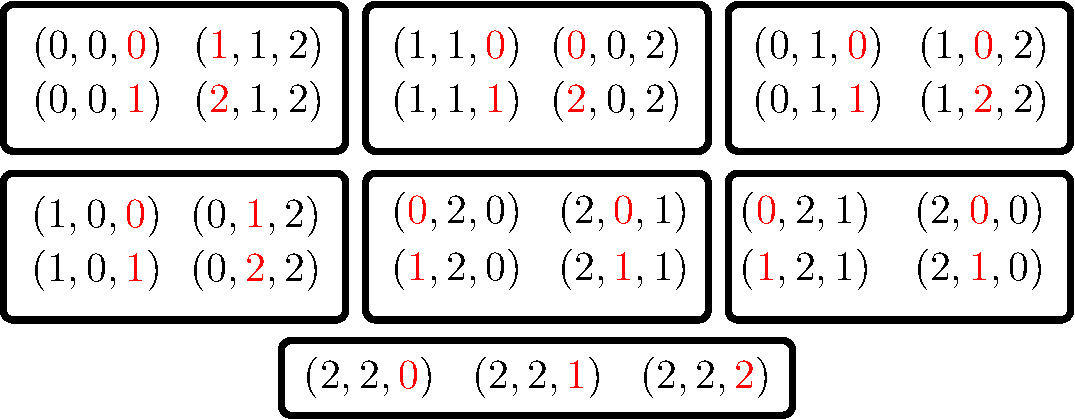
\includegraphics[width=8cm]{figs/chapter4/Alpha3}
	\caption[
	مثالی از کدگذاری بسیار منعطف با نرخ بهینه
	]{
		کدگذاری بسیار منعطف با نرخ بهینه برای
		$m=3$, 
		$\mathbb{U} = \set{ \set{1}, \set{2}, \set{3}}$,
		$k=3$.
	}
	\label{fig:eg:0}
\end{figure}
حال برای مثال اگر پیام‌ها از دسته اول باشند، فرستنده اندیس این دسته را ارسال می‌کند و گیرنده‌ای که پیام دوم را از قبل می‌داند به صورت زیر پیام جدیدی را پیدا می‌کند:
$$X_2 = 0 \Rightarrow X_1 = 0$$
و
$$X_2 = 1 \Rightarrow X_3 = 2$$


این مسئله توسط اونگ و ولامبی در
\cite{verypliable}
معرفی شده است. آن‌ها نشان می‌دهند که منعطف کردن بیشتر گیرنده‌ها برای حالت خطی هیچ بهبودی در کران ایجاد نمی‌کند ولی برای حالت کلی کران‌های اکیدا بهتری ایجاد می‌کند. برای حالتی که اندازه پیام‌ها متناهی است نسبت به حالتی که به صورت حدی بزرگ باشد نرخ‌های قابل حصول بهتری پیدا می‌کنند و  نشان می‌دهند که نرخ بهینه برای این مسئله حداقل یک است. همچنین روشی برای ساخت کدهای بسیار منعطف با الفبای بزرگتر از روی کدهای بسیار منعطف با الفبای کوچک‌تر می‌سازند.

ابزار اصلی استفاده شده در این مقاله نظریه اطلاعات است. اکثر قضایا با محاسبه آنتروپی اثبات می‌شوند. همچنین کران پایین با استفاده از
 کدهای ام‌دی‌اس (\autoref{def:mds}) به دست می‌آید.


\section{کدگذاری اندیس منعطف ترجیحی}
در 
\icod
 و 
 \picod
 گیرنده‌ها بین پیام‌های مختلف تفاوتی قائل نیستند بلکه صرفاً بازیابی هر پیامی که گیرنده از پیش نداشته باشد کافی است. بایرنه و دیگران در
\cite{byrne2023preferential}
با افزودن ترجیحات گیرنده‌ها بر روی پیام‌ها مسئله‌ی کدگذاری اندیس منعطف ترجیحی را تعریف کرده‌اند. هدف آن‌ها پیدا کردن کدهایی است که به صورت هم‌زمان نرخ ارسال و رضایت کلی گیرنده‌ها را بهبود ببخشد. برای این کار آن‌ها به دنبال مرز پارتو (\autoref{def:Pareto-boundary})
 در فضای جواب‌ها می‌گردند.
 
 یک راه‌حل 
 \transf{بروت‌فورس}{brute-force}
 برای 
 \picod
  این است که برای هر گیرنده انتخاب کنیم که کدام پیام را می‌خواهد بازیابی کند و بدین صورت مسئله را به مسئله‌ی کدگذاری اندیس تبدیل و حل کنیم و بین تمام انتخاب‌های مختلف مقدار بهینه را انتخاب کنیم.  راه‌حل‌های
 \transf{ابتکاری}{heuristic}
 در مسئله‌ی کدگذاری اندیس منعطف به جای یک 
 \transf{جست‌وجوی جامع}{exhaustive search}
به دنبال 
\transf{زیرکدهایی}{sub-codes}
هستند که در هر تکرار تعداد
\transf{ماکسیمالی}{maximal}
از گیرنده‌ها را ارضا کنند و این کار را تکرار می‌کنند تا زمانی که کل گیرنده‌ها ارضا شوند. به طور مشابه برای کدگذاری اندیس منعطف ترجیجی می‌توان با یک جست‌وجوی جامع برای تمام حالت‌های مختلف کدگذاری مقدار رضایت کلی گیرنده‌ها و طول کد را پیدا کرد که از نظر پیچیدگی محاسبه اصلا قابل قبول نیست. بایرنه و همکاران در مقاله خود یک الگوریتم ابتکاری ارائه می‌دهند که در هر تکرار به جای این‌که تنها تعداد گیرنده‌ها را حداکثر کند تابع هدفی را حداکثر کند که با دقت موازنه‌ای بین هر دو معیار برقرار می‌کند. سپس با نتایج عددی نشان می‌دهند که الگوریتم را می‌توان برای هر کدام از معیار ها بهینه کرد و خروجی نزدیک به مرز پارتو به دست آورد.

برای مدل سازی ارجحیت گیرنده‌ها از تعریف زیر استفاده می‌کنیم.
\begin{definition}
	ماتریس ترجیح
	$\boldsymbol{P}$ 
	برای یک مسئله‌ی کدگذاری اندیس منعطف ترجیحی یک ماتریس
	 $n\times m$
	 است که:
	\begin{equation}
		\boldsymbol{P} = [P_{i,j}]_{n\times m},
	\end{equation}
	به طوری که
	 $P_{i,j}\in\mathbb{R}\cup\set{\infty}$
	 ترجیح گیرنده‌ی
	 ~$i$
	 برای پیام
	  $X_j$
	  است.
	اگر یک پیام جز اطلاعات جانبی یک گیرنده باشد مقدار ترجیح آن بی‌نهایت است.
	
	در واقع ترجیح کمتر به معنی ارجحیت آن پیام است.
\end{definition}

\begin{example}
\begin{equation*}
	\boldsymbol{P} = 
	\begin{bmatrix}
		2 & \infty & 1 &\infty & 2\\
		\infty & 1 & 2 & 1 & \infty \label{eq:ppicod-instance}
	\end{bmatrix}.
\end{equation*}
\begin{figure}[H]
	\centering
	
\includegraphics[width=0.2\linewidth]{figs/chapter4/ppgraph.pdf}
	\caption[
	مثال کدگذاری اندیس ترجیحی
	]{
		مثال کدگذاری اندیس ترجیحی
		\cite{byrne2023preferential}
		}
	\label{fig:ppgraph}
\end{figure}
در واقع برعکس مدل سازی گرافی اصلی که یال برای نشان دادن اطلاعات جانبی بود اینجا برای نشان دادن نبودن اطلاعات جانبی است.
\end{example}
بایرنه و همکاران
\autoref{alg:pr-grcov}
 که بر مبنای 
 \autoref{algorithm:grcov}
  است را در مقاله خود ارائه می‌دهند. پارامتر 
 $\alpha$
 در این الگوریتم برای بهینه کردن خروجی با افزایش رضایت کلی یا افزایش نرخ کد استفاده می‌‌شود. با افزایش 
 $\alpha$
 تعداد گیرنده‌هایی که در هر تکرار ارضا می‌شوند افزایش یافته، به کد با طول کمتر می‌رسیم. در 
 \autoref{fig:alpha}
 تأثیر این پارامتر را می‌بینید.
\begin{algorithm}
	\caption[
		پوشش حریصانه‌ی ترجیحی
	\lr{PrGrCov}
	]{
		پوشش حریصانه‌ی ترجیحی
		\lr{PrGrCov($G,\alpha,\eta$)}
	}
	\label{alg:pr-grcov}
	\begin{algorithmic}[1]
		\Require
			گراف اطلاعات جانبی
		$G$
		با
		$n$
		گیرنده و
		$m$
		پیام،
		$\alpha$
		و
		$\eta$
		\Ensure
		یک کد  اندیس منعطف
		\State قرار دهید
		$\mathcal{C} \gets \emptyset$
		\State قرار دهید
		$\mathsf{SAT} \gets \emptyset$ 
		\While{$\card{\mathsf{SAT}} \neq n$}
		\State قرار دهید
		$maximal \gets \code{False}$
		\State قرار دهید
		$\mathcal{S} \gets \emptyset$
		\While{$maximal = \code{False}$}
		\State قرار دهید
		$maximal = \code{True}$
		\State
		به صورت تصادفی
		$j^{\ast}$
		را با شرط
		$j^* \in \arg \max_{j \in [1:m] \setminus \mathcal{S}} f(\mathcal{S} \cup \set{j})$
		انتخاب کنید.
		\If{$f(\mathcal{S} \cup \set{j^*}) > f(\mathcal{S})$}
		\State قرار دهید
		$\textrm{maximal} \gets \code{False}$
		\State قرار دهید
		$\mathcal{S} \gets \mathcal{S} \cup \set{j^*}$
		\EndIf
		\EndWhile
		\State قرار دهید
		 $\mathsf{SAT} \gets \mathsf{SAT} \cup W_1(\mathcal{S})$
		\State قرار دهید
		$\mathcal{C} \gets \mathcal{C} \cup \set{\mathcal{S}}$
		%\State \% Remove outgoing edges from $W_1(\mathcal{S})$:
		\State قرار دهید
		$E \gets E \setminus \set{ (u,v) \in E: u \in W_1(\mathcal{S})}$
		\EndWhile
		\State $\mathcal{C}$
		را به عنوان خروجی برگردانید.
	\end{algorithmic}
\end{algorithm}

\begin{figure}[H]
	\centering
	%\subcaptionbox{$s$ versus $\alpha$}
	{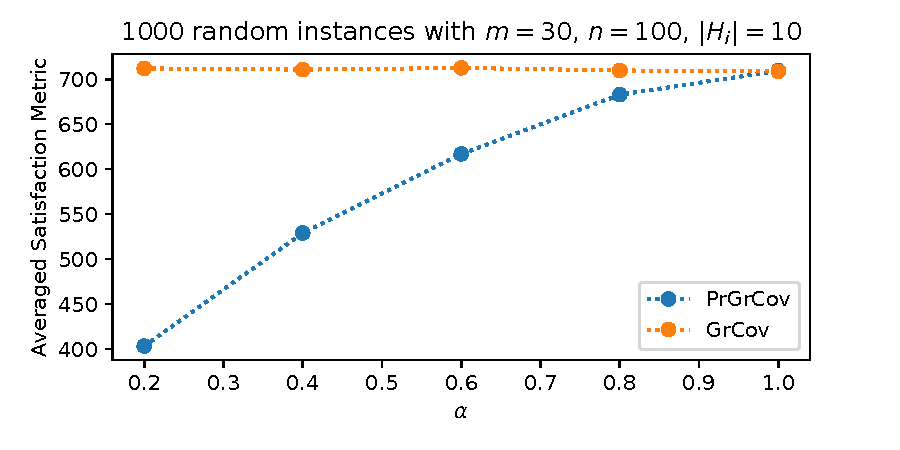
\includegraphics[width=0.4\linewidth]{figs/chapter4/cost_alpha_grcov_prgrcov.pdf}\vspace{-2ex}}
	%\subcaptionbox{$\ell$ versus $\alpha$}
	{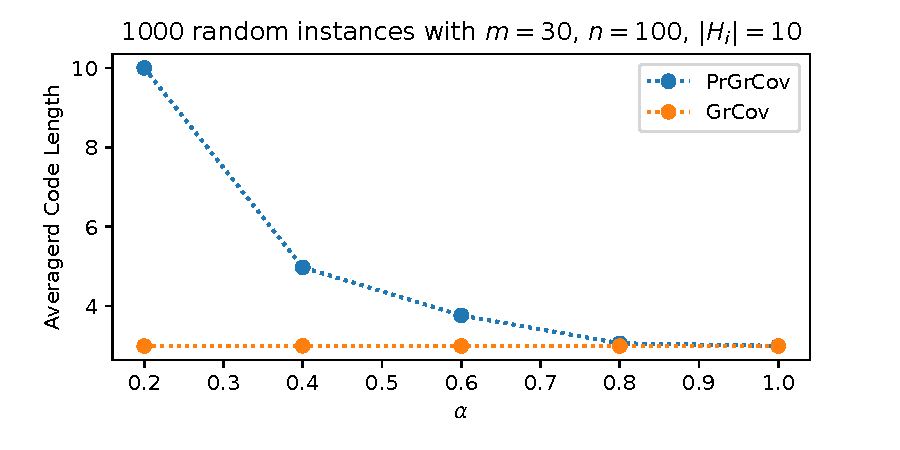
\includegraphics[width=0.4				\linewidth]{figs/chapter4/code_length_alpha_grcov_prgrcov.pdf}\vspace{-2ex}}
	\caption{
		اثر
		$\alpha$
		روی میانگین طول کد و شاخص رضایت بر روی بیش از هزار نمونه تصادفی
}
	\label{fig:alpha}
\end{figure}

\section{کدگذاری اندیس منعطف غیرمتمرکز}
ساختار مسائل مشتق شده از کدگذاری اندیس به طور کلی شامل یک فرستنده‌ی مرکزی است که با دانستن پیام‌ها و گراف اطلاعات جانبی با ارسال تعدادی پیام باعث می‌شود گیرنده‌ها به پیام‌های جدیدی دست یابند. لیو و تونینتی در
\cite{paper:Decentralized}
با حذف فرستنده‌ی مرکزی و ارسال تعدادی پیام توسط خود گیرنده‌ها، بازیابی پیام‌های جدید را به صورت غیرمتمرکز دنبال می‌کنند. در این صورت بندی، هر گیرنده تعدادی پیام ارسال می‌کند که تمام گیرنده‌های دیگر دریافت می‌کنند یعنی به جای یک تابع کدگذاری مرکزی، به هر گیرنده یک تابع کدگذاری نسبت داده می‌شود که بر اساس اطلاعات جانبی تعدادی پیام برای بقیه گیرنده‌ها ارسال کند. همچنین تابع کدگشای هر گیرنده با استفاده از اطلاعات جانبی و پیام‌های دریافتی از بقیه گیرنده‌ها پیام جدیدی را بازیابی می‌کند.

این مسئله را در واقع می‌توان حالت خاصی از مسئله کدگذاری اندیس توزیع شده
\cite{9022912}
دانست. به این صورت که به تعداد گیرنده‌ها فرستنده وجود دارد و هر فرستنده نظیر یک گیرنده است. هر فرستنده به اطلاعات جانبی گیرنده نظیر خود دسترسی دارد. هدف، کاهش تعداد استفاده از کانال ارتباطی است، به گونه ای که تمام گیرنده‌ها پیامی جدید را بازیابی کنند.

لیو و همکاران در این مقاله به دلیل پیچیدگی مسئله فقط روی دو حالت خاص آن کار می‌کنند. برای 
$m$
پیام و مجموعه‌ی
$S = \set{s_{min}, s_{min }+ 1, \ldots, s_{max}}$
مسئله‌ی 
\lr{consecutive complete–S PICOD(t)}
را به این صورت تعریف می‌کنیم: به ازای تمام حالت‌های اطلاعات جانبی ممکن از اندازه
$s \in S$
یک گیرنده در نظر میگیریم، یعنی
$n = \sum\limits_{s \in S} \binom{m}{s}$
گیرنده خواهیم داشت. همچنین مسئله‌ی
\lr{complement-consecutive complete–S PICOD(t)}
را هم به طور مشابه برای مجموعه
$S = \set{0, \ldots, m - t} \setminus \set{s_{min}, \ldots, s_{max}}$
تعریف می‌کنیم.

در این مقاله نیز از نظریه اطلاعات و ترکیبیات برای اثبات قضایا استفاده می‌شود و با استفاده از کدهای ام‌دی‌اس، کد با کران بهینه را می‌سازند. قضیه اصلی‌ای که در این مقاله اثبات می‌شود در رابطه با طول کدهای غیرمتمرکز است:
\begin{theorem}[consecutive]
	%[Optimal code-length for the decentralized consecutive complete--$S$ PICOD$(\cardi)$ with $m$ messages]
	\label{thm:consecutive_s}
	در مسئله‌ی
	\lr{decentralized complete--$S$ PICOD$(\cardi)$}
	با
	$m$ 
	پیام و
	  $S=[\smin:\smax]$
	  برای
	  $0\leq \smin \leq \smax \leq m-\cardi$
	  ، طول کد بهینه برابر است با:
	\begin{align}
		\ell^{\star}=\begin{cases}
			\frac{\binom{m}{m-\cardi}}{\binom{m}{m-\cardi}-1}  \cardi \quad \smax=\smin=m-\cardi,\\
			\min\set{\smax+\cardi, m-\smin} \quad \#
		\end{cases}
		\label{eq:thm:consecutive_s}
	\end{align}
\end{theorem}


\begin{theorem}[complement-consecutive]
	%[Optimal code-length for the decentralized complement-consecutive complete--$S$ PICOD$(\cardi)$  with $m$ messages]
	\label{thm:complement_consecutive_s}
	در مسئله‌ی
\lr{ decentralized complete--$S$ PICOD$(\cardi)$}
با
 $m$ 
 پیام
 و
 $S=[0:m-\cardi]\backslash [\smin:\smax] = [0:\smin-1]\cup[\smax+1:m-\cardi]$
 برای
 $0 < \smin \leq \smax < m-\cardi$
 ، طول کد بهینه برابر است با:
	\begin{align}
		\ell^{\star}=\min\set{m,\card{S}+2\cardi-2}.
		\label{eq:thm:complement_consecutive_s}
	\end{align}
\end{theorem}

\section{کدگذاری اندیس منعطف خصوصی}
\label{sec:privatepliable}
مسئله‌ی امنیت و حریم خصوصی در 
\icod
 از جنبه‌های مختلف بررسی شده است. دائو و همکاران در
\cite{6166891}
فرض می‌کنند که یک گیرنده دیگر نیز وجود دارد که دسترسی محدودی به اطلاعات جانبی و پیام‌های ارسال شده توسط فرستنده دارد و هدف این است که نتواند پیام جدیدی را بازیابی کند. کارموزه، فرگولی و همکاران در
\cite{8006988}
مسئله را به این شکل صورت‌بندی می‌کنند که پیام‌های ارسال شده توسط فرستنده باید به گونه‌ای باشد که هر گیرنده بتواند پیام مورد نظر خود را بازیابی کند ولی نتواند هیچ اطلاعاتی راجع به اطلاعات جانبی و پیام‌های مورد نظر بقیه گیرنده‌ها کسب کند، که شبیه به ایده‌ی
\transf{مسئله‌ی بازیابی اطلاعات خصوصی}{private information retrieval problem}
	مطرح شده در
\cite{7889028}
است.
نارایانا و همکاران در
\cite{9627083}
مسئله‌ی کدگذاری اندیس خصوصی را به این شکل صورت بندی می‌کنند که هر گیرنده فقط پیام‌های مورد نظر خودش را بازیابی کند و هیچ پیام دیگری را نتواند بازیابی کند. ساسی و راجان در
\cite{sasi2019pliable}
این تعریف را برای کدگذاری اندیس منعطف تعمیم می‌دهند. اما فقط برای حالتی که ساختار اطلاعات جانبی دایره‌ای است و هر گیرنده تنها و فقط تنها یک پیام را بتواند بازیابی کند.

لیو و تانینوتی در 
\cite{8989161}
این تعریف را بسط داده و کران‌های قابل دستیابی‌ای به دست می‌آورند.